% !TEX root = 00_main_aaai_2027.tex
% Core Appendix A: 9-benchmark boundary map, mechanism scatter, 24 within-family ladders, and reference interventions.
% Provenance: papers/analysis/answerline_delta_ci.json, papers/analysis/answerline_delta_itemlevel.json, papers/analysis/padref_control.json, papers/analysis/padref_delta_itemlevel.json.
\section{Aggregate Ranking Boundary, Ladders, and Reference Interventions}
\label{app:boundary}

This appendix formalizes teacher-forced accuracy (\tfa) and the fixed-effects decomposition, then presents the nine-benchmark aggregate ranking boundary map (Table~\ref{tab:map}), the pooled reference-perplexity correlation underlying Section~\ref{sec:mechanism} (Figure~\ref{fig:mechanism}), all twenty-four hard-side and saturated within-family model ladders (Tables~\ref{tab:ladders-hard} and~\ref{tab:ladders-sat}), and the intervention and repair sweeps (Figure~\ref{fig:sweeps}).

\paragraph{Formal definitions.}
For problem $x_i$ and tokenized worked reference $y_i^* = (t_{i1}, \dots, t_{iL_i})$, let $\hat{t}_{ij} = \arg\max_v P_M(v \mid x_i, y_{i,<j}^*)$ be scoring model $M$'s greedy next-token prediction; teacher-forced accuracy is
\begin{equation}
\mathrm{TFA}(M, x_i, y_i^*) = \frac{1}{L_i} \sum_{j=1}^{L_i} \mathbf{1}\!\left\{\hat{t}_{ij} = t_{ij}\right\}.
\end{equation}
Given a model--task score grid $s_{m,i}$ across models $m \in \{1,\dots,K\}$ and benchmark tasks $i \in \{1,\dots,N\}$, we subtract each model's overall mean $\bar{s}_{m,\cdot}$ to obtain model-centered scores $\tilde{s}_{m,i} = s_{m,i} - \bar{s}_{m,\cdot}$.
The shared item effect $\hat{\alpha}_i$ is estimated as the unweighted cross-family mean over base families $F$:
\begin{equation}
\hat{\alpha}_i = \frac{1}{|F|}\sum_{f \in F} \frac{1}{|M_f|}\sum_{m \in M_f} \tilde{s}_{m,i},
\end{equation}
and the item variance share reported in Table~\ref{tab:decomp} equals $\sum_{m,i} \hat{\alpha}_i^2 / \sum_{m,i} \tilde{s}_{m,i}^2$.
Removing both $\hat{\alpha}_i$ and the family-mean offset leaves only the per-solution residual ($5$--$11\%$ of model-centered variance on math).

\begin{table*}[t]
\centering
\caption{\textbf{Mean \tfa{} ranks models on hard benchmarks with information-dense references, weakens on code, and inverts in sign on saturated grade-school tasks.} Cross-family Spearman correlation between mean \tfa{} and accuracy ($11$--$17$ models by row; \textsc{Omni-MATH} uses a seven-model sweep and \textsc{SWE-bench Verified} eight coder models; bootstrap $95\%$ CIs) alongside the Qwen size ladder; \texttt{p-val=n/a}.
Within-family Spearmans rest on ladders of three to five models, so readers should inspect signs and counts rather than magnitudes.}
\label{tab:map}
\scriptsize
\setlength{\tabcolsep}{4pt}
\begin{tabular}{@{}llcc@{}}
\toprule
Benchmark & Regime & Cross-family $\rho$ [$95\%$ CI] & Qwen within-family $\rho$ \\
\midrule
\textsc{Omni-MATH} & Olympiad & $\mathbf{+0.86}$ $[+0.35, +1.00]$ & $+0.90$ \\
\textsc{Putnam-AXIOM} & Olympiad & $+0.60$ $[+0.17, +0.83]$ & $\mathbf{+1.00}$ \\
\textsc{Putnam-Variations} & Olympiad, contamination-proof & $+0.38$ $[-0.15, +0.73]$ & $+0.90$ \\
\textsc{HumanEval} & Code & $+0.43$ $[-0.02, +0.76]$ & $+0.80$ \\
\textsc{MATH-500} & Competition math & $+0.35$ $[-0.15, +0.71]$ & $+0.90$ \\
\textsc{MATH} (full) & Competition math, near-saturated & $+0.21$ $[-0.29, +0.61]$ & $+0.60$ \\
\textsc{GSM8K} & Grade school, saturated & $-0.25$ $[-0.71, +0.33]$ & $+0.70$ \\
\textsc{GSM8K-Platinum} & Grade school, relabeled & $-0.19$ $[-0.71, +0.41]$ & $+0.60$ \\
\textsc{SWE-bench Verified} & Agentic code, preliminary & $0.00$ ($8$ coder models) & $+1.00$ (Qwen-Coder, $n{=}4$) \\
\bottomrule
\end{tabular}
\end{table*}

\begin{figure}[t]
\centering
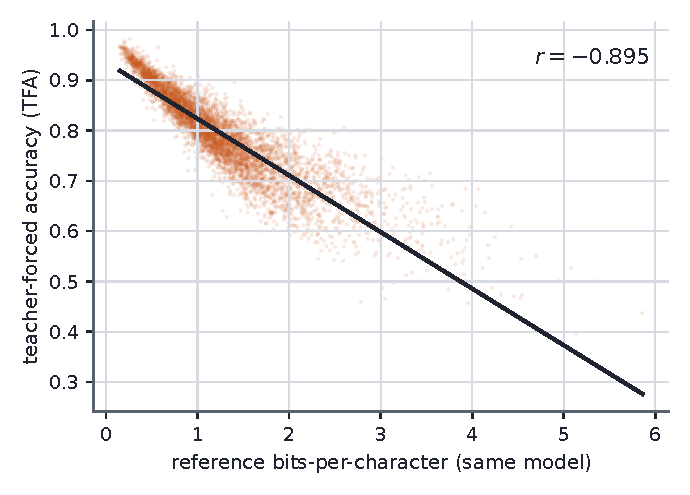
\includegraphics[width=\columnwidth]{figures/fig_mechanism.pdf}
\caption{\textbf{To first order, teacher-forced accuracy equals reference perplexity ($r = -0.895$, explaining $80\%$ of pooled variance across $6{,}000$ model--task pairs on \textsc{MATH-500}).} Per-solution \tfa{} plotted against reference bits-per-character under the same model with the least-squares linear fit.
This pooled relation is a corollary of the cross-family decomposition in Table~\ref{tab:decomp}, rather than standalone evidence, because both metrics summarize one model's predictive fit to identical text.}
\label{fig:mechanism}
\end{figure}

\paragraph{Twelve hard-side and twelve saturated family ladders.}
Tables~\ref{tab:ladders-hard} and~\ref{tab:ladders-sat} enumerate all twenty-four family--benchmark pairs across the four base families that have at least three size variants (Qwen $0.5$B--$14$B, Mistral-7B / Ministral-8B / Mistral-Small, Phi-3.5-mini / Phi-3-medium / phi-4, and OLMo-2 $7$B / $13$B / $32$B).
\textsc{Omni-MATH} is excluded from this grid because its seven-model sweep covers only Qwen.
On the three hard benchmarks, all twelve of twelve family ladders are positive ($+0.50$ to $+1.00$).
On the three saturated benchmarks, five of twelve ladders invert: Phi inverts on all three saturated benchmarks and OLMo inverts on both \textsc{GSM8K} variants, while Qwen and Mistral remain positive.
We interpret this contrast as family-specific writing-style offsets canceling within a family and driving cross-family ranking inversions once accuracy approaches ceiling; direct measurement of per-family output style remains outside this dataset, so the attribution rests on the $2.5$-fold rise in family-style variance share from \textsc{Putnam-AXIOM} ($2.9\%$) to \textsc{GSM8K} ($7.2\%$).

\begin{table}[t]
\centering
\caption{\textbf{All twelve hard-benchmark family ladders rank positively ($+0.50$ to $+1.00$).} Within-family Spearman correlations between mean \tfa{} and accuracy recomputed under the repaired answer scorer.}
\label{tab:ladders-hard}
\scriptsize
\setlength{\tabcolsep}{3pt}
\begin{tabular}{@{}lccc@{}}
\toprule
Family & \textsc{Putnam-AXIOM} & \textsc{Putnam-Variations} & \textsc{MATH-500} \\
\midrule
Qwen & $+1.00$ & $+0.90$ & $+0.90$ \\
Mistral & $+1.00$ & $+1.00$ & $+1.00$ \\
Phi & $+1.00$ & $+0.50$ & $+0.50$ \\
OLMo & $+0.50$ & $+0.50$ & $+1.00$ \\
\bottomrule
\end{tabular}
\end{table}

\begin{table}[t]
\centering
\caption{\textbf{Five of twelve saturated-benchmark family ladders invert in sign.} Within-family Spearman correlations under the repaired answer scorer; asterisks ($^*$) mark inverted ladders (Phi on all three saturated sets and OLMo on both \textsc{GSM8K} sets).}
\label{tab:ladders-sat}
\scriptsize
\setlength{\tabcolsep}{3pt}
\begin{tabular}{@{}lccc@{}}
\toprule
Family & Full \textsc{MATH} & \textsc{GSM8K} & \textsc{GSM8K-Platinum} \\
\midrule
Qwen & $+0.60$ & $+0.70$ & $+0.60$ \\
Mistral & $+1.00$ & $+1.00$ & $+1.00$ \\
Phi & $-1.00^*$ & $-0.50^*$ & $-0.50^*$ \\
OLMo & $+1.00$ & $-0.50^*$ & $-0.50^*$ \\
\bottomrule
\end{tabular}
\end{table}

\paragraph{Reference interventions and repair sweeps.}
Figure~\ref{fig:sweeps} illustrates why heuristic token reweighting cannot repair \tfa{} while deeper completion prefixes strengthen verification without matching the extracted-answer check.
Across the twelve models with per-token hit vectors on \textsc{MATH-500} (whose baseline ranking correlation is $\rho = +0.126$), weighting token positions by $(\mathrm{pos}/n)^\gamma$ holds near $+0.154$ at $\gamma{=}1$, collapses to $+0.014$ at $\gamma{=}4$ and $-0.007$ at $\gamma{=}8$, and flips sign to $-0.371$ when restricted to the last four tokens.
Similarly, residualizing reference perplexity out of \tfa{} drops ranking correlation from $+0.13$ to $-0.17$ and yields an item-level partial correlation of $+0.09$ (raw $-0.11$), while seven earlier exploratory variants (inverse document frequency weighting, surprisal weighting, token masking, and variants) all produced correlations $\le 0$.
In the \texttt{P-L1} boilerplate control, replacing worked derivations with identical boilerplate text padded to mean reference length produces mean \tfa{} $= 0.464$ across seventeen models while destroying ranking ($\rho = -0.11 \; [-0.57, +0.35]$; twelve-model item-paired worked-minus-padded $\Delta\rho = +0.41 \; [+0.35, +0.46]$), ruling out token-count shrinkage as the cause of the answer-line collapse ($\Delta\rho = +0.24 \; [+0.12, +0.33]$ on $12$ models; $+0.33 \; [-0.16, +0.81]$ across $17$ models).

\begin{figure}[t]
\centering
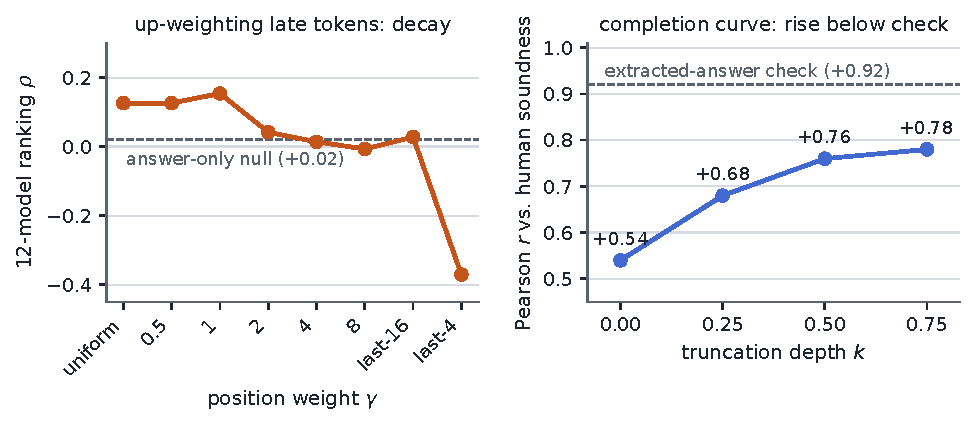
\includegraphics[width=\columnwidth]{figures/fig_sweeps.pdf}
\caption{\textbf{Reweighting late reference tokens drives \tfa{} ranking negative ($-0.37$), whereas completion depth raises soundness validity toward---but never past---the extracted-answer check ($+0.92$).} Left: $12$-model \textsc{MATH-500} ranking Spearman under position weights $(\mathrm{pos}/n)^\gamma$; the decay misses our pre-registered null call by overshooting into a sign flip.
Right: anchor-set Pearson correlation of the Qwen2.5-14B completion curve across truncation depth $k \in \{0, 0.25, 0.50, 0.75\}$ (Spearman profile is non-monotone: $+0.47, +0.32, +0.48, +0.46$).}
\label{fig:sweeps}
\end{figure}
